\section{Optimal Control}\label{chap:optimal}
In this chapter, we tackle the problem of \textit{Quantum Optimal Control}. We control our quantum system by sending some (classical)electromagnetic pulse into a cavity. An obvious question arises: what pulse shape needs to be sent to achieve a particular operation on our quantum system? 

It turns out that this questions does not have an easy answer. In the rest of the chapter we'll try to give an answer using an algorithm called \textbf{\textit{GRAPE}}.

\subsection{GRAPE}
Although in some cases we can calculate the desired pulse analytically\footnote{As seen in appendix \ref{appen:annalytic}}, most of the time this isn't an option. Often, we need to use numeric means to find an optimal pulse. To find the desired pulse numerically, we can model our system on a classical computer and simulate what happens when you send a pulse. Using the results of the simulation, we try to change the pulse until we get the desired effect.

So what's GRAPE then? GRAPE in an acronym for \textit{\textbf{GR}adient \textbf{A}scent \textbf{P}ulse \textbf{E}ngineering}. When we model a quantum system, in our case, a qubit interacting with a cavity, we can model the physical information about the system using the Hamiltonian of the system. We can split the Hamiltonian into two. There's the Hamiltonian that nature gives us, of how a qubit behaves and how it interacts with its surrounding. And there's the Hamiltonian we control, using electromagnetic control pulses. We can send any possible pulse shape. To account for that fact, we treat the pulse as a function of time, as a step-wise constant function. The pulse is, essentially, just an array of many variables, and we want to find the values that give the desired result. This is a classical case of an optimization problem. To optimize the values, we set a cost function that tells us how "good" the current pulse is.

In principle, we could use a brute-force search and check every possible pulse until we find one that minimizes the cost function. This method is inefficient. A better way to optimize the function is by calculating also the \textit{gradient} of the cost function, and using an optimization algorithm\footnote{The \textbf{L}imited memory \textbf{B}royden–\textbf{F}letcher–\textbf{G}oldfarb–\textbf{S}hanno (L-BFGS-B) algorithm (the \textbf{B} is since it could handle simple box constraints) in our case. It's a quasi-newton iterative method for nonlinear optimization problems. We "feed" into it the cost function and gradient}, to find the minimum of the function efficiently.
\begin{figure}[H]
    \centering
    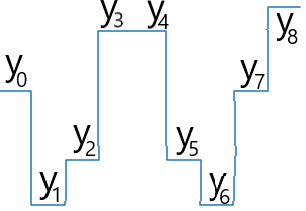
\includegraphics[width=0.3\columnwidth]{step-wise_example.png} % TODO: Change the image
    \caption{Example of a step-wise constant function as an array of numbers}
    \label{fig:step-wise-const}
\end{figure}
\subsection{The Cost Function}
When our desired operation is to prepare our quantum system in a predetermined state, a good figure of merit of how close our system is to the desired state is given by the \textbf{fidelity}. The fidelity is a measure of the "closeness" of two quantum states, The fidelity is $0$ when the two states are orthogonal, and $1$ if they are identical. The fidelity is given by the magnitude of the \textit{overlap} between the two states squared\footnote{Assuming both states are pure states and not mixed states}.

\begin{equation} \label{def:fid}
F (\psi_1, \psi_2) = \abs{\braket{\psi_1}{\psi_2}}^2
\end{equation}
The \textit{infidelity}, $1 - F$ between the two states, can be conveniently used as the cost function in our optimization procedure\footnote{Since we want to maximize the fidelity, we want to minimize the infidelity}. Given an initial state and a target state, along with the Hamiltonian and pulse information, we want to be able to calculate the fidelity for any given pulse. To do so, we need to solve Schr\"{o}dinger's equation for the pulse
\begin{equation}
i\hbar\frac{d}{dt}\ket{\Psi (t)} = \hat{H}\ket{\Psi (t)}
\end{equation}
In the previous chapter we characterized the Hamiltonian of the system (equations (\ref{eq:JC-hamiltonian}) and (\ref{eq:dispersive-hamiltonian})),
% TODO: Add explanation about that there are multiple different pulses and throughout the chapter we're referring to a single pulse which is most of the time not the case
\begin{equation} \label{eq:hamiltonianl_form}
H (t) = H_0 + \sum_k{\epsilon_k (t) H_k} % Maybe put the next part before the part about the Schrodinger equation
\end{equation}
where $H_0$ is the (time-independent) Hamiltonian of the system without the drives (given, for example, from the Jaynes-Cummings model). Each $\epsilon_k (t)$ is the amplitude as a function of time of the control drive pulses, and each $H_k$ is the (time-independent)Hamiltonian describing the interaction between the control pulse and the rest of the system. We call these Hamiltonians the \textit{drive hamiltonians}. Our goal with GRAPE is to find optimal $\epsilon_k (t)$.

On each constant step of the amplitude functions $\epsilon_k (t)$, the entire Hamiltonian is constant. Luckily, the solution of the Schr\"{o}dinger equation for a constant Hamiltonian is easily solved by
\begin{equation}
\hat{U} (t) = e^{-\frac{i}{\hbar}\int_{T_0}^{T_1}H (t)dt}
\end{equation}
If we choose $T_0$ and $T_1$ as the end points of a step of the Hamiltonian, the total Hamiltonian of the system is constant so the integral is just a simple multiplication by $T_1-T_0$ which we'll write as $\delta t = T_1 - T_0$. The solution becomes
\begin{equation}
\hat{U} (t) = e^{-\frac{i\cdot \delta t}{\hbar}H (t)}
\end{equation}

In order to calculate the solution over the entire pulse we need to solve for the first step, then find the solution by the end of that time-step, and use it as the initial condition for the next time step, repeating for each time step. The solution until the $N^{th}$ time step is simply the product of the previous solutions for each time step
\begin{equation}\label{eq:U_def_prod}
\hat{U}_N (\epsilon (t)) = \prod_{k = 1}^N\hat{U}_k (\epsilon (t))
\end{equation}
With $\hat{U} (\epsilon)$ in hand, we can calculate the evolution of the state over the entire pulse
\begin{equation}
\ket{\Psi_{final}} = \hat{U} (\epsilon)\ket{\Psi_{initial}}
\end{equation}
This way, if we want to calculate the fidelity after applying the drives, we can simply calculate the fidelity between the target state and the final, calculated state
\begin{equation} \label{eq:fidelity_sim}
F (\epsilon (t)) = F (\Psi_{target}, \Psi_{final}) = \abs{\bra{\Psi_{target}}\hat{U}_N\ket{\Psi_{initial}}}^2
\end{equation}

As mentioned, if we want to optimize the cost function efficiently we'll need to calculate the gradient of the cost function along with the cost function itself.

\subsection{The Gradient}
For simplicity, we'll first derive the gradient of the \textit{overlap}
\begin{equation} \label{def:overlap}
c = \braket{\Psi_{target}}{\Psi_{final}} = \bra{\Psi_{target}}\hat{U}\ket{\Psi_{initial}}
\end{equation}
We can then get the fidelity by noting that $F = \abs{c}^2$. We want to differentiate the overlap by each control parameter. To do so, note that $\hat{U}$ is defined as:
\[ 
\hat{U} = \hat{U}_N \hat{U}_{n-1}...\hat{U}_2 \hat{U}_1
\]
And when differentiating by a control parameter only one $\hat{U}_k$ is affected,
\[
\frac{\partial c}{\partial \epsilon_k} = \bra{\Psi_{target}}\hat{U}_N \hat{U}_{N-1} ... \hat{U}_{k+1}\frac{\partial \hat{U}}{\partial \epsilon_k} \hat{U}_{k-1} ...\hat{U}_2 \hat{U}_1\ket{\Psi_{initial}} 
\]
We can write that for a constant Hamiltonian (from Schr\"{o}dinger's equation)
\[
    \hat{U}_k = e^{-\frac{i\cdot \delta t}{\hbar}H (t)}
\]
And approximate the derivative $\frac{\partial \hat{U}_k}{\partial \epsilon_k}$ in the limit of small $\delta t$ by writing
\begin{equation*}
    \frac{\partial \hat{U}_k}{\partial \epsilon_k} \approx -\frac{i\cdot \delta t}{\hbar}\frac{\partial H}{\partial \epsilon_k} \cdot e^{-\frac{i\cdot \delta t}{\hbar}H (t)} = -\frac{i\cdot \delta t}{\hbar}\frac{\partial H}{\partial \epsilon_k} \hat{U}_k
\end{equation*}

Theoretically, we have everything we need to calculate the gradient, but it's still rather complex computationally ($o (N^2)$ complexity). A different method can be used to reduce the computational overhead.

The derivative of the cost function by a control parameter of the pulse has become
\begin{equation} \label{eq:cost_init_deriv}
    \frac{dc}{d\epsilon_k} = -\frac{i\cdot \delta t}{\hbar} \underbrace{\bra{\Psi_{target}}\hat{U}_N \hat{U}_{N-1}... \hat{U}_{k+1}}_{\bra{\psi_{bwd}^{ (k+1)}}}\frac{dH}{d\epsilon_k} \underbrace{\hat{U}_{k} ...\hat{U}_2 \hat{U}_1\ket{\Psi_{initial}}}_{\ket{\psi_{fwd}^{ (k)}}}
\end{equation}
Where we defined two arrays, $\bra{\psi_{bwd}}$ and $\ket{\psi_{fwd}}$, the multiplication components before and after the derivative of H
\begin{equation} \label{eq:cost-function-b/fwd}
    \frac{\partial c}{\partial \epsilon_k} =  -\frac{i\cdot \delta t}{\hbar}\bra{\psi_{bwd}^{ (k+1)}} \frac{\partial H}{\partial \epsilon_k} \ket{\psi_{fwd}^{ (k)}}
\end{equation}
We can see from \ref{eq:cost_init_deriv} that 
\[   
\ket{\psi_{fwd}^{ (k)}} = 
     \begin{cases}
       \ket{\psi_{init}} &\quad\ k=0\\
       \hat{U}_k \ket{\psi_{fwd}^{ (k-1)}} &\quad\ otherwise\\
     \end{cases}
\]
\[   
\ket{\psi_{bwd}^{ (k)}} = 
     \begin{cases}
       \ket{\psi_{targ}} &\quad\ k=N+1\\
       \hat{U}_k^{\dag{}} \ket{\psi_{bwd}^{ (k+1)}} &\quad\ otherwise\\
     \end{cases}
\]
Now all we need is to do $2N$ calculations in the beginning ($N$ for $bwd$ and $N$ for $fwd$), and then calculating the actual gradient using equation \ref{eq:cost-function-b/fwd}. This improves the computation complexity from $o (N^2)$ to $o (N)$, while the memory complexity stays $o (N)$.

It's important to note that $c$ is not the fidelity, but the overlap. We can get the fidelity from $c$ by
\[
F = |c|^2
\]
since $c$ might be complex this derivative is a bit less trivial than it might seem. We can write $c (\vec{\epsilon})$ as $a (\vec{\epsilon}) + b (\vec{\epsilon})i$, where $a, b \in R$ and we get that 
\[
\frac{\partial F}{\partial \epsilon_k} = \frac{\partial |c|^2}{\partial \epsilon_k} = \frac{\partial |a+bi|^2}{\partial \epsilon_k} = \frac{\partial (a^2 + b^2)}{\partial \epsilon_k} = 2 (a\frac{\partial a}{\partial \epsilon_k} + b\frac{\partial b}{\partial \epsilon_k})
\]
We can notice that $c (\frac{\partial c}{\partial \epsilon_k})^* = a\frac{\partial a}{\partial \epsilon_k} + b\frac{\partial b}{\partial \epsilon_k} + (ab - \frac{\partial a}{\partial \epsilon_k}\frac{\partial b}{\partial \epsilon_k})i$. More importantly, we can see that the real part of that expression is exactly what we need. Putting it all into one formula we get
\begin{equation} \label{eq:fidelity_gradient_final}
    \frac{\partial F}{\partial \epsilon_k} = 2\cdot \Re{c (\frac{\partial c}{\partial \epsilon_k})^*}
\end{equation}
Now all you need is to plug \ref{eq:cost-function-b/fwd} and \ref{def:overlap} into \ref{eq:fidelity_gradient_final} and you got your gradient :)

Let's do a little test now to see that everything is working well. The simplest pulse you can send is the pulse that takes the qubit from being in state $\ket{0}$ to state $\ket{1}$, where the transition frequency is set to $1$Ghz (hence the period is $1$ns). We discussed this situation in appendix \ref{appen:annalytic} so we know how the solution should look like. Running our GRAPE code with some random initial pulse we get
\begin{figure}[H]
    \centering
    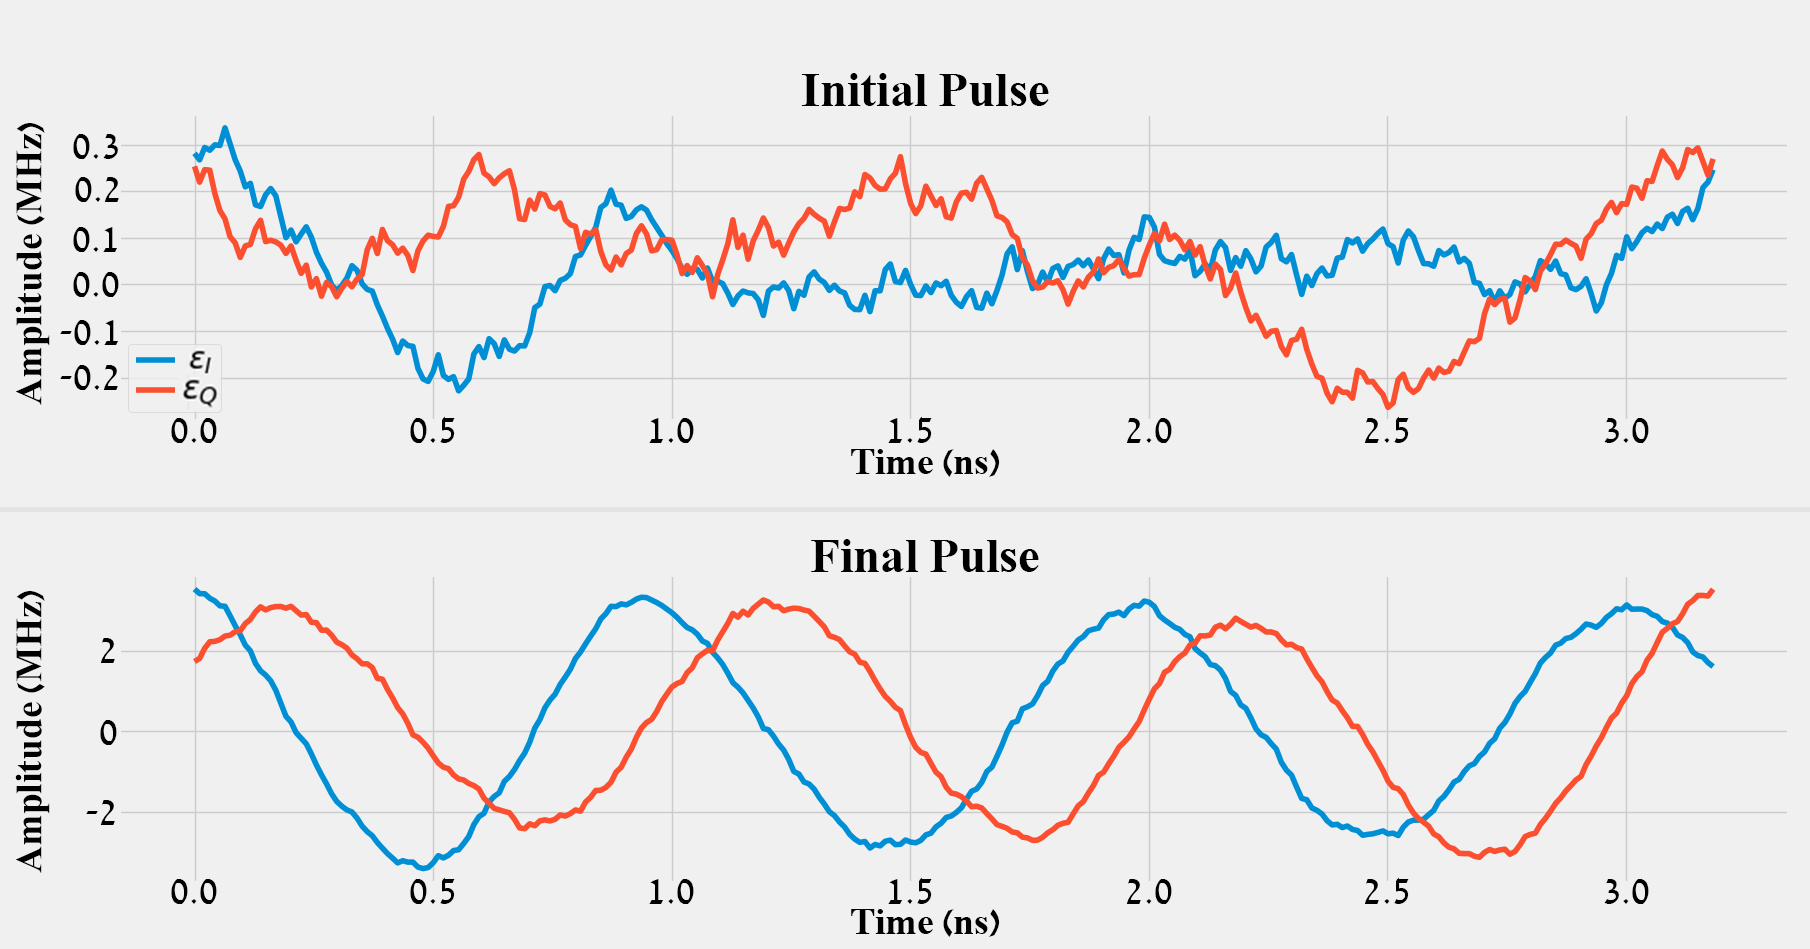
\includegraphics[width=0.8\columnwidth]{Results/No-Constraints-single-qubit/pulses-prettier.png}
    \caption{Pulses solution for $\ket{0} \rightarrow \ket{1}$. Each color is a different microwave control pulse of the system, I and Q. They are the real and imaginary parts of the calculated wave in appendix \ref{appen:annalytic} }
    \label{fig:GRAPE-first-example}
\end{figure}
Amazing! From some random initial pulse we got sinusoidal waves with $1$Ghz frequency, just as predicted in appendix \ref{appen:annalytic}.

Before we get too excited, there are a couple of things weird with this pulse. The first, more obvious problem, is that although the waves are sin and cos as expected, they're still pretty jagged-y, there is some randomness on top of the wave and it's not as smooth as we expected. This is since small random changes don't really change the final result\footnote{The noise cancels itself out}. In addition, high-frequency components generated  by the computer do not have an effect in reality. This is due to the limited bandwidth of our pulse generator and RF circuitry.

Another problem, that is not immediately obvious, we can only see if we look at the population graph of the qubit over the duration of the pulse. We expect the graph to start at $1$ and end at $0$ for $\ket{0}$ and start at $0$ and end at $1$ for $\ket{1}$. Let's look at that graph for the initial random pulse and for the optimized pulse
\begin{figure}[H]
    \centering
    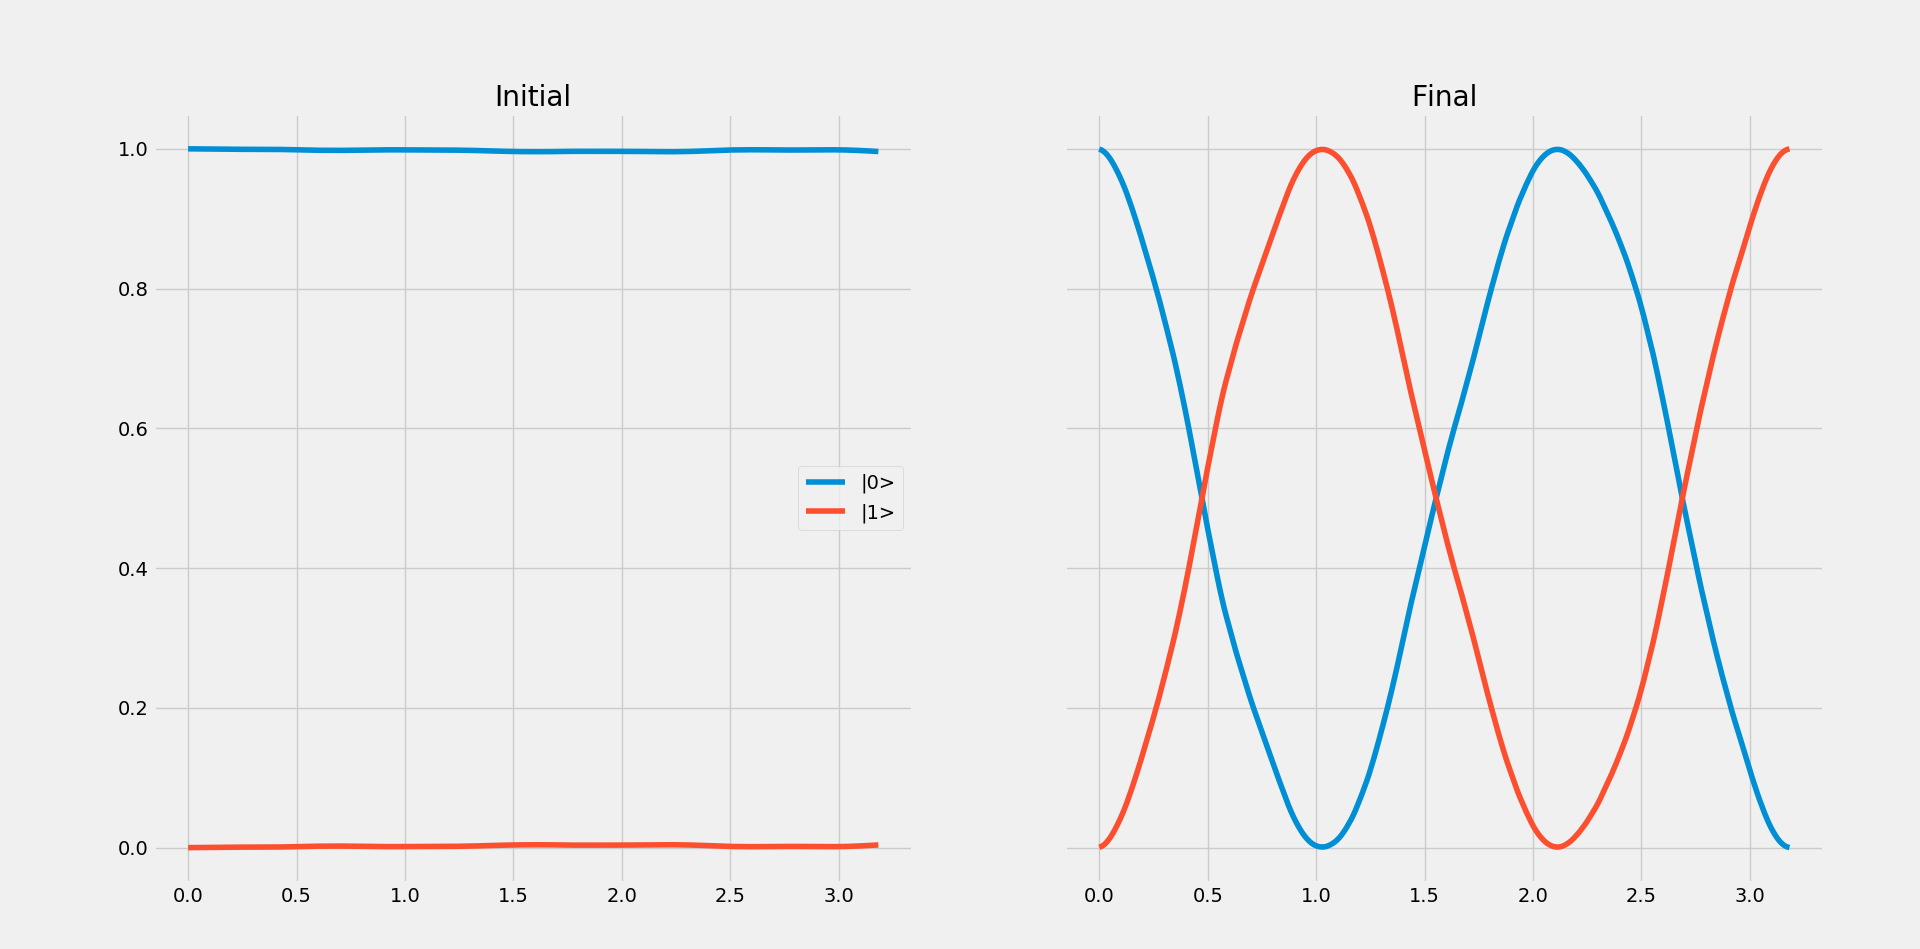
\includegraphics[width=1\columnwidth]{Results/No-Constraints-single-qubit/level-population-pretty2.png}
    \caption{Population of qubit levels over pulse duration. Before the optimization, the state of the qubit (population of ground and excited states) almost did not change at all. After the optimization, the qubit goes from state $\ket{0}$ to $\ket{1}$ to $\ket{0}$ to $\ket{1}$, doing some unnecessary back and forth between the states}
    \label{fig:GRAPE-first-example-level-population}
\end{figure}
As expected, the initial random pulse doesn't change the pulse almost at all. The optimized pulse on the other hand is problematic. The population of $\ket{0}$ for example, goes from 0 to 1 and then goes back to 0 to start over again. Ideally, the population will change from 0 to 1 (and vice-versa) smoothly, only once.

This happens because the amplitude of the optimized pulse is too big. As we defined the optimization, the algorithm doesn't care that the population acts weirdly in the middle of the pulse as long as it ends at the desired state.

To solve these problems (and more we'll talk about), we introduce \textit{constraints} to the algorithm.
% \footnote{I'll give a quick note just to be honest, since this is such a simple case, GRAPE works pretty well even without any constraints. I've carefully crafted conditions so that the final pulse wouldn't be smooth and so the level population would go crazy. This is what you'll see normally in more complex examples but I didn't want to go with a complex example since it would just complicate things without giving any real benefit}

\subsection{Constraints}
% Unfortunately, we live in the real world, and in the real world we can't just make ultra-fast frequency pulses with the energy of the sun. It's impossible because of the limitation of our devices. The computer doesn't care for the limitation of the devices, That's why we need to add constraints to the cost function.
Since instruments have physical limitations, for example, on the maximum amplitude of a pulse, we must add constraints on the computer calculations to not exceed these limitations.

We define a set of constraints on the solution ${g_i \ge 0}$, and associate a Lagrange multiplier $\lambda_i$ to each constraint\footnote{In an ideal optimized pulse, $g_i = 0$}. \newline
Our goal is to minimize 
$$1 - F (\vec{\epsilon}) + \sum_i \lambda_i g_i (\vec{\epsilon})$$
Let's add a constraint to each of the most problematic physical limitations.
\subsubsection{Limiting the Amplitude}
This is the most obvious physical limitation. We can't generate pulses with infinite energy, so we have to restrict it. There are two ways we can do so, the first is to create a hard cut-off amplitude. No matter what, the amplitude will never go above this amplitude. We usually want this cut-off to be the  maximal output amplitude of our pulse generator. But normally we don't want our generator to work at its absolute limit\footnote{Not only that it might damage the device, with stronger pulses the non-linear optical effects increase}, so we can add also a soft amplitude maximum by "rewarding" the cost function to stay at a lower amplitude. Let's see how we would implement such a thing, starting with the hard cut-off.

Instead of controlling and changing the amplitude ($\vec{\epsilon}$) directly, we'll introduce a variable $\vec{x}$ and relate them as
\[
    \vec{\epsilon} = \epsilon_{max}\tanh{\vec{x}}
\]
As you probably guessed, $\epsilon_{max}$ is the maximum amplitude of the pulse.
Since the optimization algorithm can only change $\vec{x}$, the amplitude of the pulse will always be between $-\epsilon_{max}$ and $\epsilon_{max}$. Unfortunately, this changes the gradient of the cost function since we now want the derivative with respect to $\vec{x}$ instead of $\vec{\epsilon}$. We can relate the two
\[
\frac{\partial F}{\partial \vec{x}} = \frac{\partial F}{\partial \vec{\epsilon}}\frac{\partial \vec{\epsilon}}{\partial \vec{x}} = \frac{\epsilon_{max}}{\cosh^2{\vec{x}}} \ \frac{\partial F}{\partial \vec{\epsilon}}
\]
We can use the derivative $\frac{\partial F}{\partial \vec{\epsilon}}$ we got from \ref{eq:fidelity_gradient_final} and simply calculate $\frac{\epsilon_{max}}{\cosh^2{\vec{x}}}$ and we again have the gradient.\footnote{Since $\tanh (x)$ is a positive monotonic transformation it preserves the locations of the maxima of the function. This means that in practice we can just ignore the new derivative}

% For the soft limitation, there are two limitation we can make, linear and non-linear. The linear goal is for general preference of low amplitude pulses and the non-linear is if you have a specific $\epsilon_{max,soft}$ that you want to be well below of (You can use both or either one depends on your desired pulse properties). We'll start with the linear case since it's simpler.
% TODO: NON-LINEAR
For the soft amplitude penalty all we want is that \textit{bigger amplitudes} $\Rightarrow$ \textit{bigger cost function}. Since our algorithm seeks to minimize the cost function, this will lead to the overall amplitude being smaller. The way we do so is simple, we can define a constraint $g_{amp}$ that sums all the amplitudes of the steps of the pulse, so
\[
    g_{amp} = \sum_k |\epsilon_k|^2
\]
Still, since it is added to our cost function we need to find the gradient of the penalty as well. In this case it's rather simple since it's a basic parabola
\[
    \frac{\partial g_{amp}}{\partial \epsilon_k} = 2\epsilon_k
\]
and now we have all we need in order to add this penalty to our cost function.\footnote{We can also create non-linear soft amplitude constraint. With such constraint we can set a soft maximum we want to stay well below of. We won't show how to do so}% Let's move on to the non-liner penalty.

% For the non-linear amplitude penalty we have a slightly different goal in mind
% TODO: Add here the non linear amplitude penalty


\subsubsection{Limiting Bandwidth and Slope}
The next limitation is the maximum frequency our AWG can create because the device can't change the voltage instantaneously. Again, like we had with the amplitude limit, there are 2 types of limits we can make, hard and soft. Let's start with the hard limit.

We have some frequency $ \omega_{max} $ which is the maximum frequency that our AWG can generate. To make sure that our simulation doesn't produce such a pulse we can go from time space to the frequency space with a Fourier transform
\[
    \vec{\epsilon} = (DFT)^{-1} \vec{x}
\]
The numerical optimization algorithm controls $\vec{x}$ which is in the frequency space. Now if we want to limit the frequency we can simply set to 0 any frequency that is above our maximum frequency
\[
    x (\omega > \omega_{max}) = 0
\]
The gradient of the new cost function is simply the Fourier transform of x
\[
    \frac{\partial \vec{x}}{\partial \epsilon_k} = (DFT) \frac{\partial \vec{\epsilon}}{\partial \epsilon_k}
\]
And we know $\frac{\partial \vec{\epsilon}}{\partial \epsilon_k}$ from previous sections.
It's important to note that the hard cut-off of the amplitude and the hard cut-off of the frequency do not work together since one is in time domain and one is in frequency domain. This is not much of a problem since we can compensate with the soft limits that do work well together (since they require adding to the cost function instead of changing coordinates). In my simulations I use the amplitude hard limit instead of the frequency one since it is easier to work with.

For the soft limits, we're limiting the slope (derivative) of the pulses and not the frequency directly. The slope of a step function is simply $\epsilon_{k+1} - \epsilon_{k}$, we want to limit the size of the slope so we'll look at the expression $|\epsilon_{k+1} - \epsilon_{k}|^2$ instead. Summing all the slopes (to get an overall slope size of the entire pulse) we get the expression\footnote{Note that we have a problem at the edges since the slope of the end points is not well defined, we'll fix this problem later but for now we just ignore the last point $k=N$}
\begin{equation}\label{eq:g_slope}
    g_{slope} = \sum_{k=0}^{N-1} |\epsilon_{k+1} - \epsilon_{k}|^2
\end{equation}{}
Unlike the amplitude, since the slope of the boundaries is not well defined we'll have the edges defined differently than the center of the pulse. The gradient of $g$ in the center is a simple derivative, notice that each $\epsilon_k$ appears only twice in the sum
\[
    \frac{\partial g_{slope}}{\partial \epsilon_k} = 4\epsilon_k - 2 (\epsilon_{k+1} + \epsilon_{k-1})
\]
It's nice to see that the expression looks like how'd you numerically estimate the second derivative, since the gradient of the slope (which is the derivative) is the second derivative. Now we need to define the gradient at the edges, you can see that the derivative of $\epsilon_k$ depends on his neighbors on both sides. Since the first and last element of the pulse don't have 2 neighbors they are treated a little differently. each of the edges appears only once in the sum \ref{eq:g_slope} unlike the others that appear twice, we can simply take the derivative of that one term and get
\begin{align*}
    &\frac{\partial g_{slope}}{\partial \epsilon_0} = 2 (\epsilon_1 - \epsilon_0) \\
    &\frac{\partial g_{slope}}{\partial \epsilon_N} = 2 (\epsilon_N - \epsilon_{N-1})
\end{align*} 
Now, before we continue, we'll add another small constraint that will also solve the problem of the slope at the boundaries. It might seem weird at first, but we want to pulse to zero-out at the edges. This is since our AWG device can't immediately start a pulse with some amplitude, it can't get from 0 to that amplitude instantaneously (for the same reason we limit the slope in the first place). This could be achieved by simply setting the first and last steps of the pulse and their gradient to 0.
\[
    \epsilon_0 = \epsilon_N = \frac{\partial \ \text{Cost}}{\partial \epsilon_0} = \frac{\partial \ \text{Cost}}{\partial \epsilon_N} = 0
\]
This solves the problem we were trying to solve we were having with the slope at the boundaries, since the gradient is 0 at the edges and does not depend on its neighbors.% We can move on to the non-linear limitation now.

% As we mentioned earlier, the goal of the non-linear limitation is when we have a specific bandwidth to be well below off, the could be achieved thanks to the fact that exponents grow really fast
% \[
%     Add\ equation\ here
% \]
% TODO: Add here but more importantly change how is the goal of the non-linear limitation explained.

Now that we have both amplitude constraint and bandwidth constraint we can use them to get a nice, smooth solution, that any wave generator would be happy to produce
\begin{figure}[H]
    \centering
    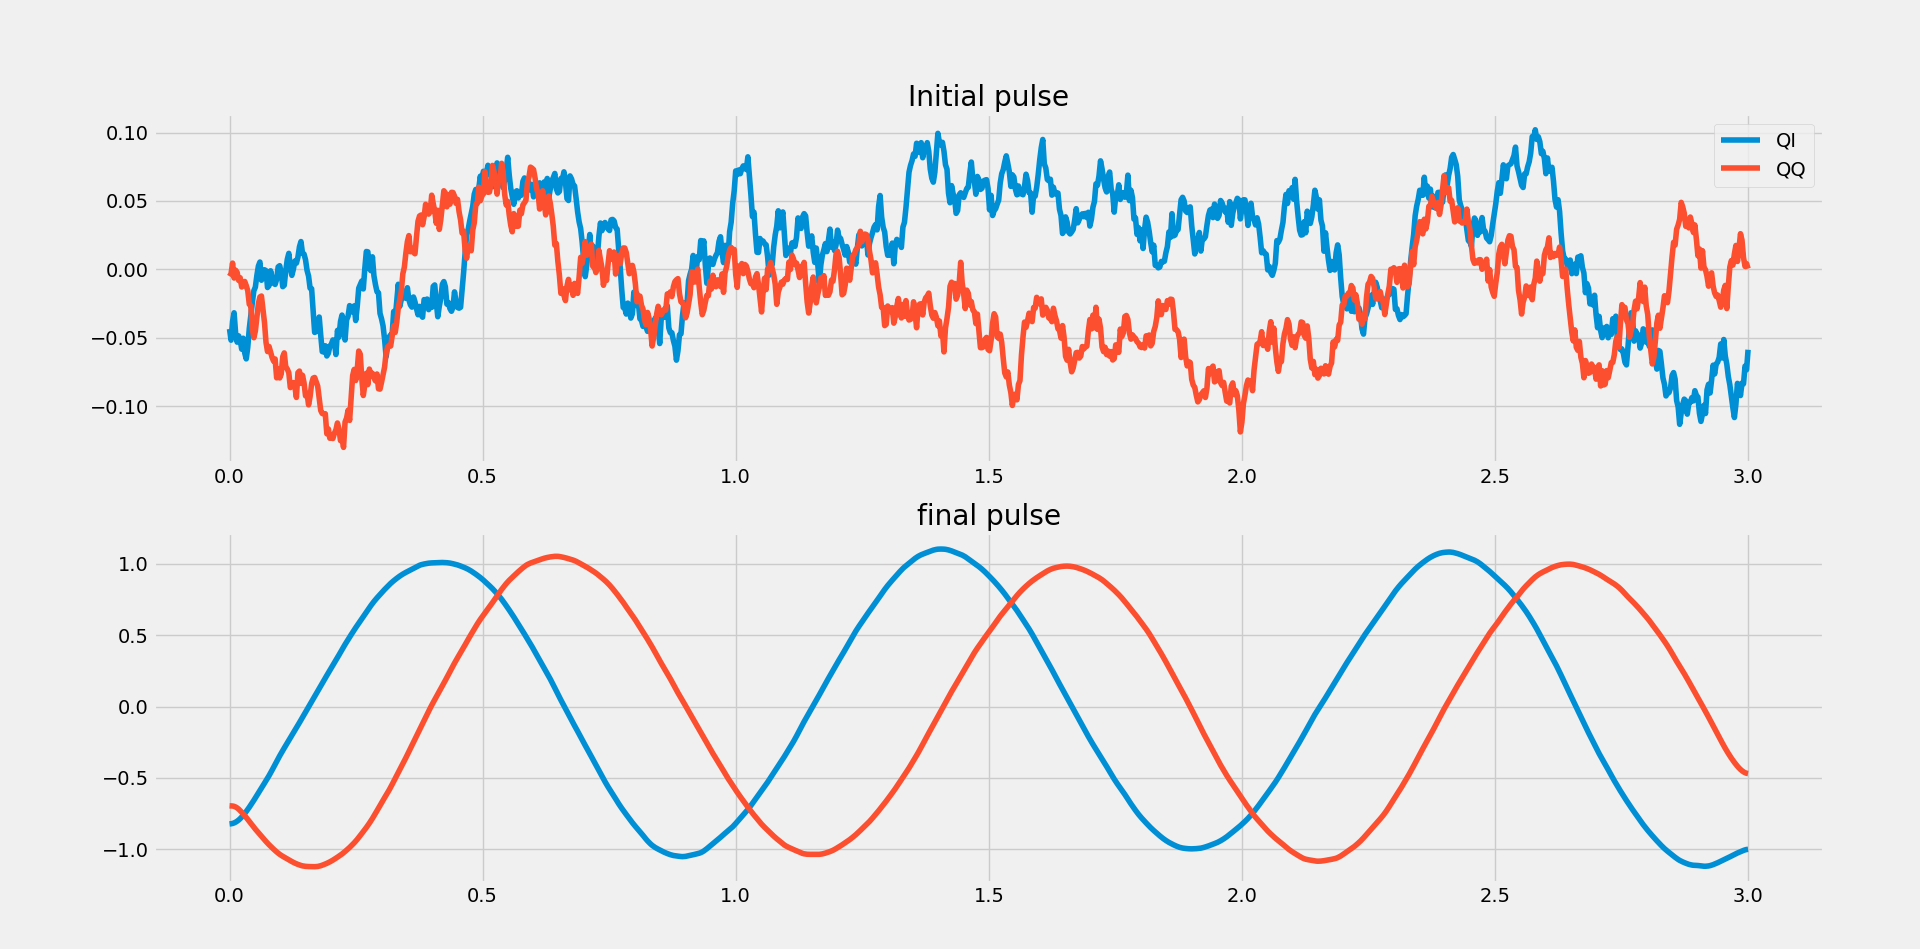
\includegraphics[width=1\columnwidth]{Results/qubit-band-amp-const/pulses.png}
    \caption{Control pulses before and after GRAPE optimization with amplitude and bandwidth constraints}
    \label{fig:band-amp-const-qubit}
\end{figure}
The pulse is exactly what we expect it to be. More importantly, if we look at the population graph of the levels, it does exactly what we want, go from state $\ket{0}$ to state $\ket{1}$ without going back and forth.
\begin{figure}[H]
    \centering
    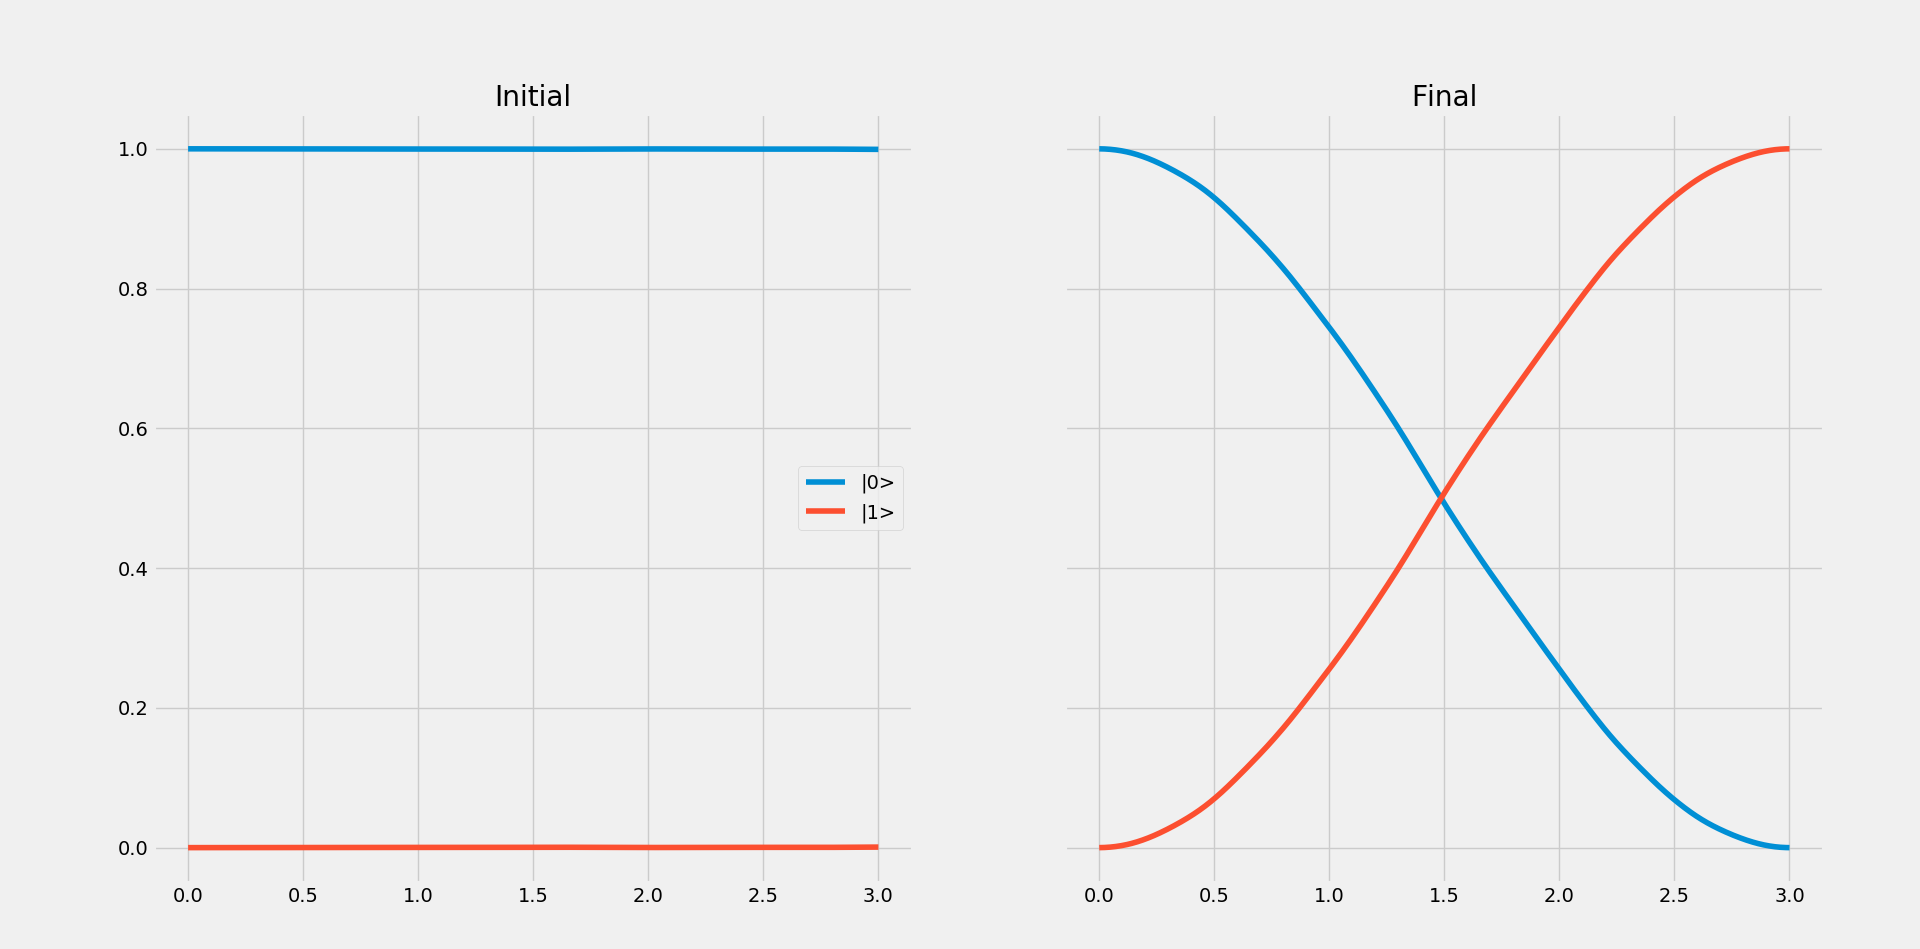
\includegraphics[width=1\columnwidth]{Results/qubit-band-amp-const/level-population.png}
    \caption{Population of qubit levels over pulse duration. Before the optimization, the state of the qubit (population of ground and excited states) almost did not change at all. After the optimization, the qubit goes from state $\ket{0}$ to $\ket{1}$}
    \label{fig:band-amp-const-level-population}
\end{figure}

Another interesting visualisation of the success of this pulse is the path of the qubit on the Bloch sphere over time (see the last section in chapter \ref{chap:quantum-optics}). Plotting the populations on the Bloch sphere we get 
\begin{figure}[H]
    \centering
    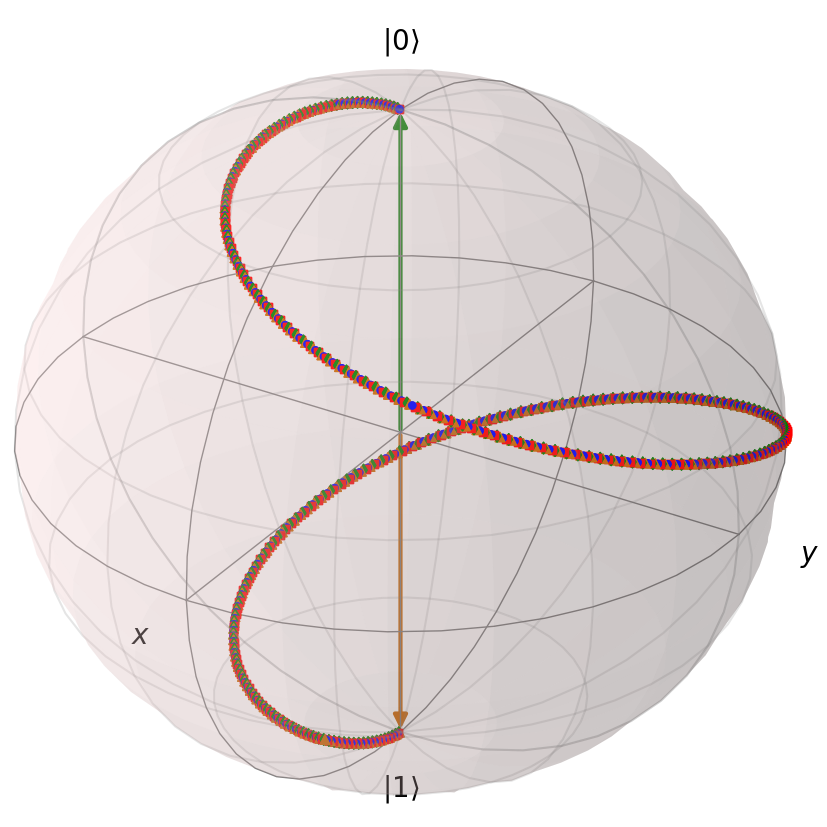
\includegraphics[width=0.4\columnwidth]{Results/qubit-band-amp-const/Bloch-qubit.png}
    \caption{Path of the qubit along the Bloch sphere. The qubit goes from state $\ket{0}$ to state $\ket{1}$, preforming one loop on the sphere, the arrows represent the initial state and the target state, and the points represent the path of the state of the qubit}
    \label{fig:band-amp-const-blcoh}
\end{figure}
As you can see, the path of the qubit isn't a straight line, but some loop, completing a full rotation around the $\hat{z}$ axis. This is explained by the fact that the base Hamiltonian of the qubit is $\omega \hat{\sigma}_z$, where $\hat{\sigma}_z$ is the Pauli matrix Z. This matrix corresponds to rotation of the Bloch sphere around the $\hat{z}$ axis. This is why we can think of the entire Bloch sphere as always rotating with frequency $\omega_0$ around the $\hat{z}$ axis, this is why a "straight" path is actually one that does one loop around the $\hat{z}$ axis.

\subsubsection{Limiting Pulse Duration}
As much as I wouldn't mind waiting a few nanoseconds longer for the qubit operation to end, the qubit itself isn't as patient as me. A state-of-the-art qubit would last, at most, few hundred microseconds (and that's a very optimistic estimation). We simply don't have the time to wait for the operation to end if we want to run some complicated quantum circuit. This is why we want to add a constraint on the \textit{duration} of the pulse. This way, if we set the total duration of the pulse to longer than the shortest possible pulse, it would find the shorter pulse and the rest of the pulse will change nothing (see figure \ref{fig:dur-penelty})

% give the pulse 5ns to finish, and a solution of 3ns exists, the optimization algorithm would (hopefully) find the 3ns solution and the rest of the time until the end of the duration will do nothing.

The constraint is fairly straight forward, add a penalty for any time a fidelity of 1 isn't achieved. Put into an equation we get
\[
    g_{duration} = \sum_{i = 0}^{N-1} (1 - F_i)
\]
Where $F_i$ is the fidelity at time step $i$.

We can rather simply calculate the fidelity at any given time since they are already calculated in order to find the fidelity in the last time step. We can simply modify the loop that calculates the final state into giving the fidelity at each time step and sum the results. 
% TODO: Maybe remove some of the technical details about the code and the implementation

Luckily for us, the calculation of the gradient is also pretty simple. The gradient of the fidelity at each time step is calculated the same as the gradient of the fidelity we calculated in the beginning of the chapter\footnote{note that $\epsilon_k$ only appears in the expression for $F_i$, if $i > k$, so the sum starts at $i = k$}
\[
    \frac{\partial g_{duration}}{\partial \epsilon_k} = -\sum_{i = k}^{N-1}\frac{\partial F_i}{\partial \epsilon_k}
\]
% TODO: I think I can find a more efficient solution, Got to check this in the code and ask serge for his opinion

The pulse duration constraint works nicely to complete the other constraints. Without this constraint, the pulse will "try" to use all it's time to get the result we desire. When running the algorithm without the constraint we can get problems if the duration we gave to the pulse is too long or too short. With this constraint on, we can simply give the algorithm a duration that we know for sure is more then the minimum required time, and the algorithm will simply use the minimum time it needs, and no more. On the other hand, if we didn't have the amplitude (and bandwidth) constraints, the algorithm might find that it's best to just give a super-strong pulse for a tiny amount of time, but that's not physically possible as we discussed. This is why we can think of the constraints working together to "box in" the pulse into an ideal "size".

If we run GRAPE now, with all the constraints together, and look at the population of all the level over the duration of the pulse, we get\footnote{This is a rather extreme case where the total duration of the pulse is around three times longer then the minimum duration. This was done purposefully to demonstrate the point.}
\begin{figure}[H]
    \centering
    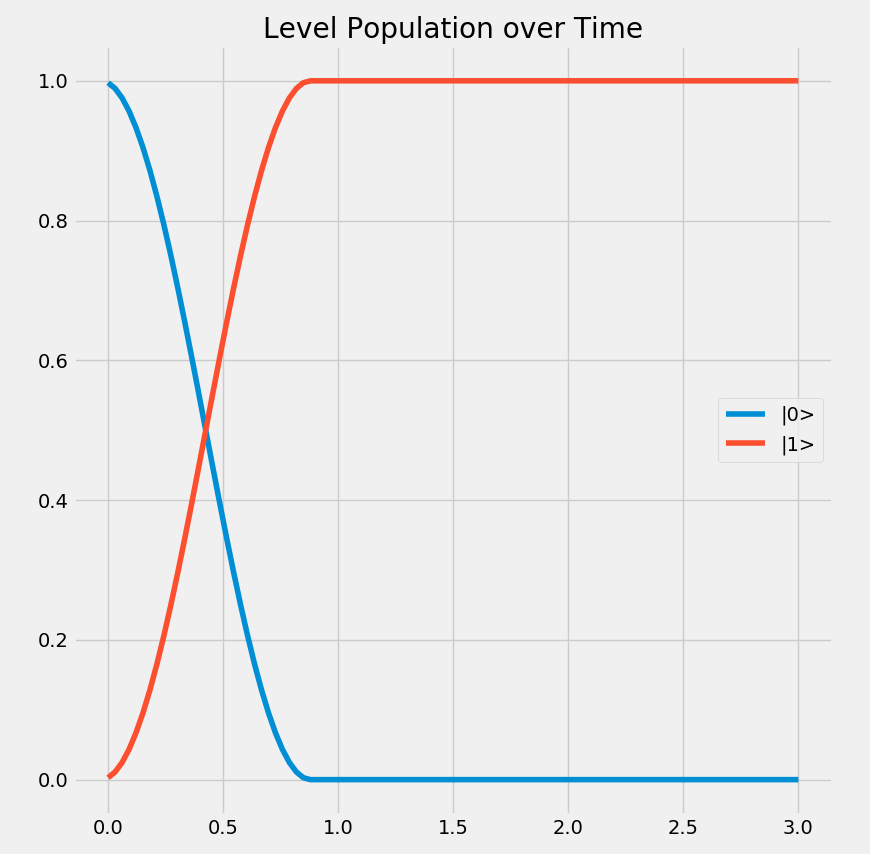
\includegraphics[width=0.5\columnwidth]{Results/duration-constraint/level-population.png}
    \caption{Level population of each state as a function of time over the duration of the pulse.}
    \label{fig:dur-penelty}
\end{figure}

As expected, we get exactly what we want, the pulse uses the least amount of time that it needs and then stop. This way, if we pick a long duration for the pulse, instead of the pulse trying to fill the entire time at a very low amplitude, or do several of loops before arriving at the target, the qubit simply takes exactly the amount of time that it needs to get to the desired state under all of the constraints and then stops.

\subsection{Implementing Qubit Operations with GRAPE}

\subsubsection{DRAG - Imperfect Qubits} \label{sec:DRAG}
When we did all of our calculation on the qubit we didn't include one detail, it's really hard to create a true two-level system. In the way our qubits are implemented, there are actually more than two levels. It's not a two level system but we treat it as one. Since the higher levels are off-resonance, we can often just ignore them. However, there is some probability of the higher levels getting populated by high-frequency components of our pulses. The shorter our pulses are, the more these higher  levels excitation occur. We will prevent those so-called leakage errors by using \textbf{D}erivative \textbf{R}emoval via \textbf{A}diabatic \textbf{G}ate (DRAG) pulses. We can generate those pulses by including more than two levels in our algorithm and changing the Hamiltonian a little bit so it accounts for the off-resonance higher levels.

Before we continue to implement DRAG, let's see if the third level really is that much of a problem. We run a simulation of GRAPE just as we did before but this time with three levels instead of two, and the third level should start and end at 0 population. We get after running GRAPE
\begin{figure}[H]
    \centering
    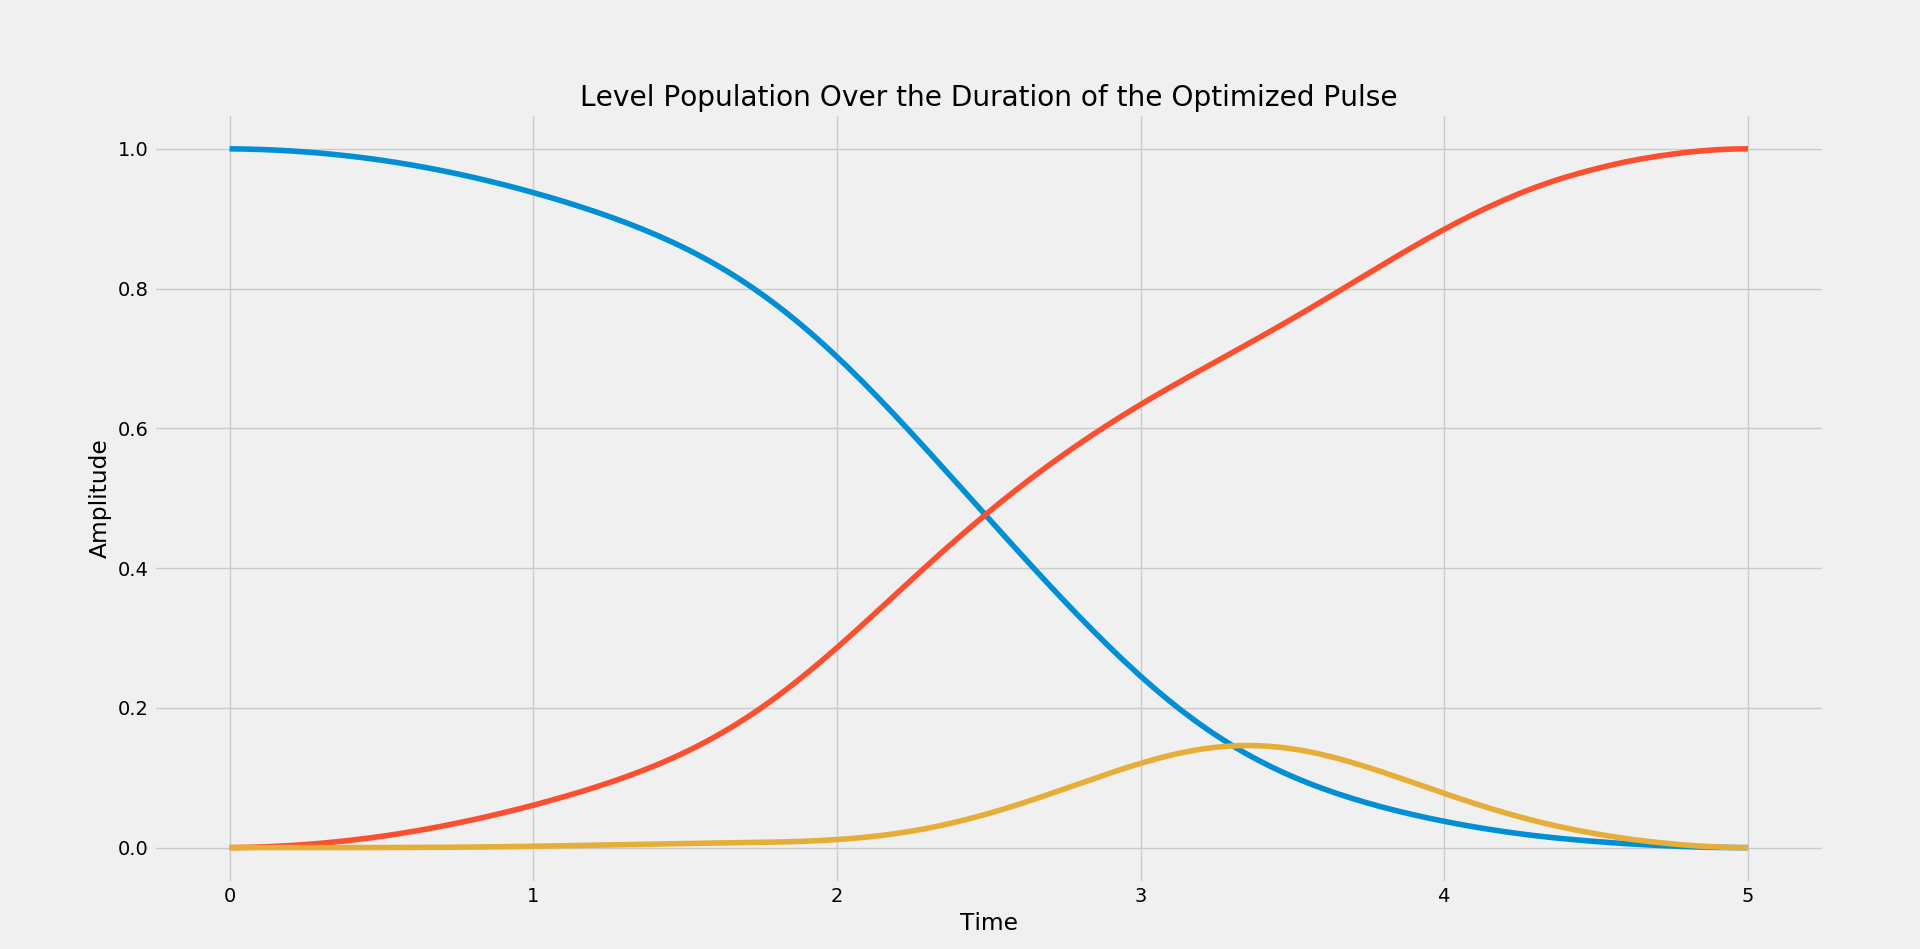
\includegraphics[width=1\columnwidth]{Results/Before-Drag/level-population-pretty.png}
    \caption{Level population of the 3-level "qubit" over the duration of the pulse calculated by the GRAPE algorithm we have so far}
    \label{fig:before-DRAG}
\end{figure}
Well yes, the forbidden level did start and end at $0$ population\footnote{If you decrease the anharmonicity you would also have final forbidden level population, which is a more serious problem}, but in the middle the qubit really became a 3 level system with the population of the forbidden level being really dominant around time $3.5$! We can't simply replace the qubit with a 3 level system and make the target of the third level always 0 and call it a day. \textbf{We can't treat higher levels as just more "qubit" levels}, they are unwanted and we need to give them a penalty so the probability of being in a higher level would be always almost zero and change only a tiny bit. There are many ways we could implement such a penalty, the most obvious way is by simply making the probability to be in an higher level into a penalty, summing over all time we get (We'll call the third level of the qubit $\ket{f}$ to not be confused with the $\ket{3}$ Fock state (photon number state))\footnote{If we wanted to accounted for higher levels we can sum over the sum for each level}
\[
    g_{forbidden} = \sum_{i=0}^{N - 1} \abs{\braket{f}{\psi_{fwd}^{ (i)}}}^2 
\]
We already have $\psi_{fwd}^{ (i)}$ that we calculated earlier, so for so good.

Now moving to to complex part of DRAG, the gradient. Let's again define the overlap
\[
    c_{f} = \sum_{i=0}^{N - 1} \braket{f}{\psi_{fwd}^{ (i)}}
\]
now to calculate the gradient we'll derive over $\epsilon_k$
\[
    \frac{\partial c_{f}}{\partial \epsilon_k} = \frac{\partial}{\partial \epsilon_k}\sum_{i=0}^{N - 1}  \braket{f}{\psi_{fwd}^{ (i)}} = \sum_{i=0}^{N - 1} \frac{\partial}{\partial \epsilon_k} \braket{f}{\psi_{fwd}^{ (i)}}
\]
recall that $\psi_{fwd}^{ (i)} = \hat{U}_i \cdot \hat{U}_{i-1} \cdot ... \cdot \hat{U}_1 \ket{\psi_{initial}}$, $\hat{U}_k$ only appears for $i > k$, so we can start the sum from $i = k$. We'll also expand $\psi_{fwd}^{ (i)}$ into what it is and get
\[
    \frac{\partial c_{f}}{\partial \epsilon_k} = \sum_{i=k}^{N - 1} \frac{\partial}{\partial \epsilon_k} \bra{f}\hat{U}_i \cdot ... \cdot \hat{U}_0 \ket{\psi_{initial}}
\]
the only element that depends on $\epsilon_k$ is $\hat{U}_k$, so we can rearrange the equation as
\begin{align*}
    \frac{\partial c_{f}}{\partial \epsilon_k} &= \sum_{i=k}^{N - 1} \bra{f}\hat{U}_i \cdot ...\cdot \frac{\partial \hat{U}_k}{\partial \epsilon_k} \cdot ... \cdot \hat{U}_0 \ket{\psi_{initial}} \\
    &= \sum_{i=k}^{N - 1} \bra{f}\hat{U}_i \cdot ...\cdot i \cdot \delta t\frac{\partial H_k}{\partial \epsilon_k} \hat{U}_k\cdot ... \cdot \hat{U}_0 \ket{\psi_{initial}} \\
    &= i \cdot \delta t \sum_{i=k}^{N - 1} \bra{f}\hat{U}_i \cdot ... \cdot \hat{U}_{k+1} \cdot \frac{\partial H_k}{\partial \epsilon_k}\ket{\psi_{fwd}^{ (k)}}
\end{align*}
Now just to keep everything simple and maintainable, we'll define
\[
    \bra{\phi_{bwd}^{ (i,k)}} = \bra{f} \hat{U}_i \cdot ... \cdot \hat{U}_{k+1}
\]
The equation for the overlap now becomes
\[
    \boxed{\frac{\partial c_{f}}{\partial \epsilon_k} = i \cdot \delta t \sum_{i=k}^{N - 1} \bra{\phi_{bwd}^{ (i,k)}} \frac{\partial H_k}{\partial \epsilon_k} \ket{\psi_{fwd}^{ (k)}}}
\]
Now we got all we need to calculate the penalty of the occupying the higher level and it's gradient. This isn't a perfect solution though, for $N$ time steps we need to do $o (N^2)$ calculations to get $\bra{\phi_{bwd}^{ (i,k)}}$. This slows down the calculation considerably\footnote{it makes to calculation run around 100 times slower, pretty bad considering it's just a penalty} and there is a lot of overhead in the way we calculated $\bra{\phi_{bwd}^{ (i,k)}}$. We can use a smarter way to calculate it.

Consider a function, very similar to  $\bra{\psi_{bwd}}$ we had earlier (in fact, it's the same function minus multiplying by the target state on the left)
\[
    \psi_{bwd}^{ (k)} = \hat{U}_N\hat{U}_{N-1}...\hat{U}_{k+2}\hat{U}_{k+1}
\]
taking the inverse of the resulting matrix we get
\[
    (\psi_{bwd}^{ (i)})^{-1} = \hat{U}_{i+1}^{-1}\hat{U}_{i+2}^{-1}...\hat{U}_{N-1}^{-1}\hat{U}_{N}^{-1}
\]
by multiplying the two matrices we get (defining their product as $\phi_{bwd}$)
\[
    \phi_{bwd}^{ (i,k)} = (\psi_{bwd}^{ (i)})^{-1} (\psi_{bwd}^{ (k)}) = (\hat{U}_{i+1}^{-1}\cdot...\cdot \hat{U}_{N}^{-1}) (\hat{U}_N\cdot...\cdot \hat{U}_{k+1}) = \hat{U}_{i}\cdot...\cdot \hat{U}_{k+1}
\]
This is exactly what we wanted! from this we'll define
\[
    \bra{\phi_{bwd}^{ (i,k)}} = \bra{f}\phi_{bwd}^{ (i,k)}
\]
remember that $\psi_{bwd}$ was already calculated from the gradient calculation, taking the inverse of $\psi_{bwd}$ isn't affected by how many time steps there are, also the multiplications between $\psi_{bwd}$, $ (\psi_{bwd})^{-1}$ and $\bra{f}$ isn't dependent on the amount of time steps, so the entire calculation is $o (N)$ complexity.

Let's run now the algorithm and get some results
\begin{figure}[H]
    \centering
    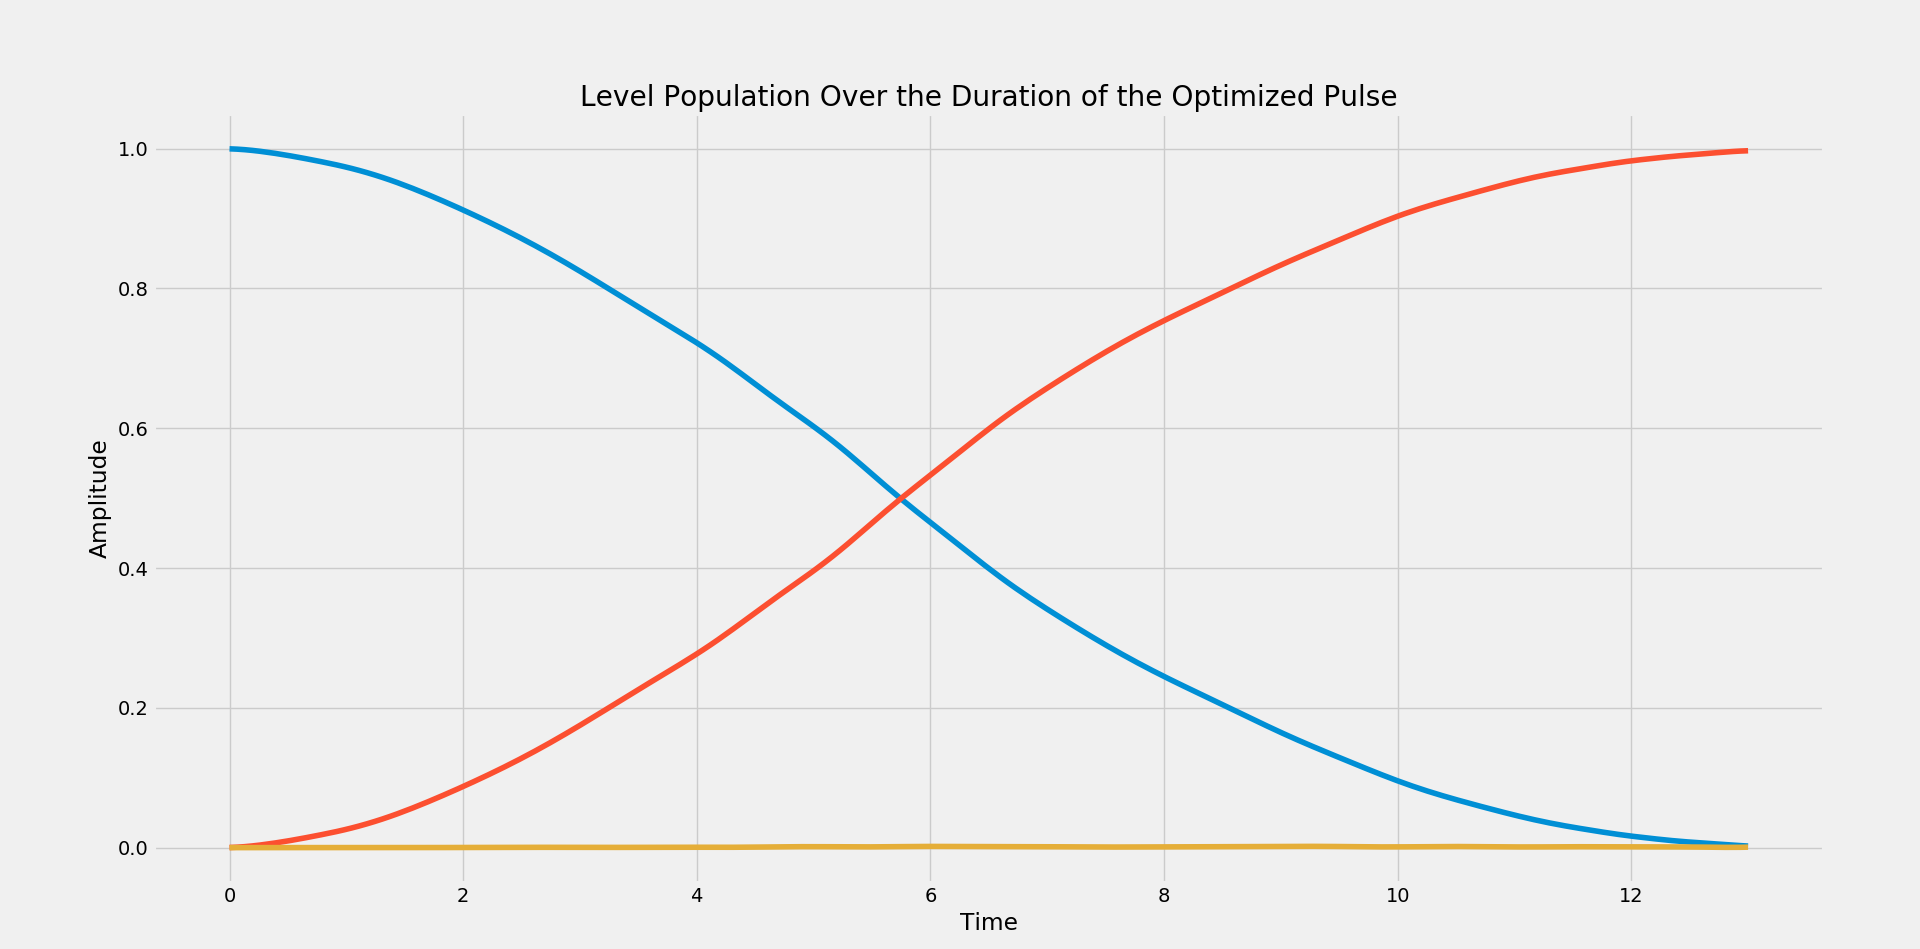
\includegraphics[width=1\columnwidth]{Results/DRAG/level-population2.png}
    \caption{Level population of the "qubit" over the duration of the pulse that was found by the GRAPE algorithm, with all the penalties turned on, including the DRAG penalty.}
    \label{fig:sDRAG-results}
\end{figure}
Nice! state $\ket{0}$ goes directly to $1$, $\ket{1}$ goes directly to $0$ and the forbidden level is barley changed throughout the pulse (the fidelity gotten from this pulse is around $99.9\%$, so pretty good).

I think that we talked enough about the qubit for now, let's move the the other half of the system, the cavity.

\subsection{Implementing Cavity Operations}
\subsubsection{Limiting the photon number} 
\centerline{\say{Hilbert space is a big place.}}
\centerline{- Carlton Caves}
Here's the thing about the cavity levels, there are infinite amount of them. We can make an assumption that the cavity only has $N$ levels, but it is still possible that something happens in the higher levels that may affect the physical result. We want to make sure that everything interesting is contained in the $N$ levels that we have.

This is quite similar to what we did in the previous section with DRAG, we want to put a penalty on the higher levels. Still, there are two main differences. The first, is that there are much more than one or two extra levels, and as we've seen, the method we used in the previous uses very heavy computation and we can't do it for so many levels. The other difference is that we care less about if some higher level is occupied for a part of the pulse. In the cavity there are higher levels and they're all likely to be but \textbf{the reason we're limiting the cavity levels is for computing reasons, not physical ones}. Unlike the cavity, we really want the qubit dynamics to involve only two levels, so it makes sense that we'll use a different penalty to limit the photon number.

The idea is this, we'll define $n_{ph}$ as the highest level we want the cavity to have. Now let's calculate what will happen if the cavity will have another level, for a total of $n_{ph} + 1$. Ideally, nothing will change, the new level should start at 0 probability and end at 0 probability with no change in between. If there is a change, will add a penalty to the pulse, so in the next iteration there will be less of a change. We can do so for any level higher than one, so instead of using only $n_{ph} + 1$ we'll some over $n_{ph} + k$ for reasonable amount of k's.

We'll define $F_{n_{ph} + k}$ as the fidelity if there were $n_{ph} + k$ levels. Putting the idea into a formula we get that the new cost function is given by
\[
    Cost = \sum_{k=0}^{N} F_{n_{ph} + k} (\vec{\epsilon}) - \sum_i \lambda_i g_i (\vec{\epsilon})
\]
We can double enforce the penalty if we add a constraint making sure there is no change in the fidelity for different levels
\[
    g_{ph} = \sum_{k_1 \ne k_2} (F_{n_{ph} + k_1} - F_{n_{ph} + k_2})^2
\]
The gradient of which is simply the gradient of which is simply
\[
    \frac{\partial g_{ph}}{\partial \epsilon_k} = 2 \sum_{k_1 \ne k_2} [ (F_{n_{ph} + k_1} - F_{n_{ph} + k_2}) (\frac{\partial F_{n_{ph} + k_1}}{\partial \epsilon_k} - \frac{\partial F_{n_{ph} + k_2}}{\partial \epsilon_k})]
\]
and everything in this expression was previously calculated (they're simply the derivatives of the fidelity and the fidelity itself).

It's important to note that while it might be tempting to leave $n_{ph}$ at a small value so there will be less to calculate (the size of the matrices grows with $n_{ph}^2$), there is good reason to use a high values of $n_{ph}$. Bigger $n_{ph}$ oscillate at higher frequency (since the cavity is simply a harmonic oscillator), so it's possible to use shorter pulses, and since keeping qubit alive is really a major problem, keeping the pulses short is important to be able to accomplish the most with the time we have with the qubit before it dies.
% TODO: Need to go over the last paragraph and check it with Serge to make sure I'm not making anything up

Lets see what happens if we run the transmon-cavity code. We'll only look at the resulting population graph after the optimization. I warn you that the graph is a bit cluttered. You shouldn't look at any specific details or any specific curve, I didn't put a legend explaining what each curve is. We'll look at it then discuss

\begin{figure}[H]
    \centering
    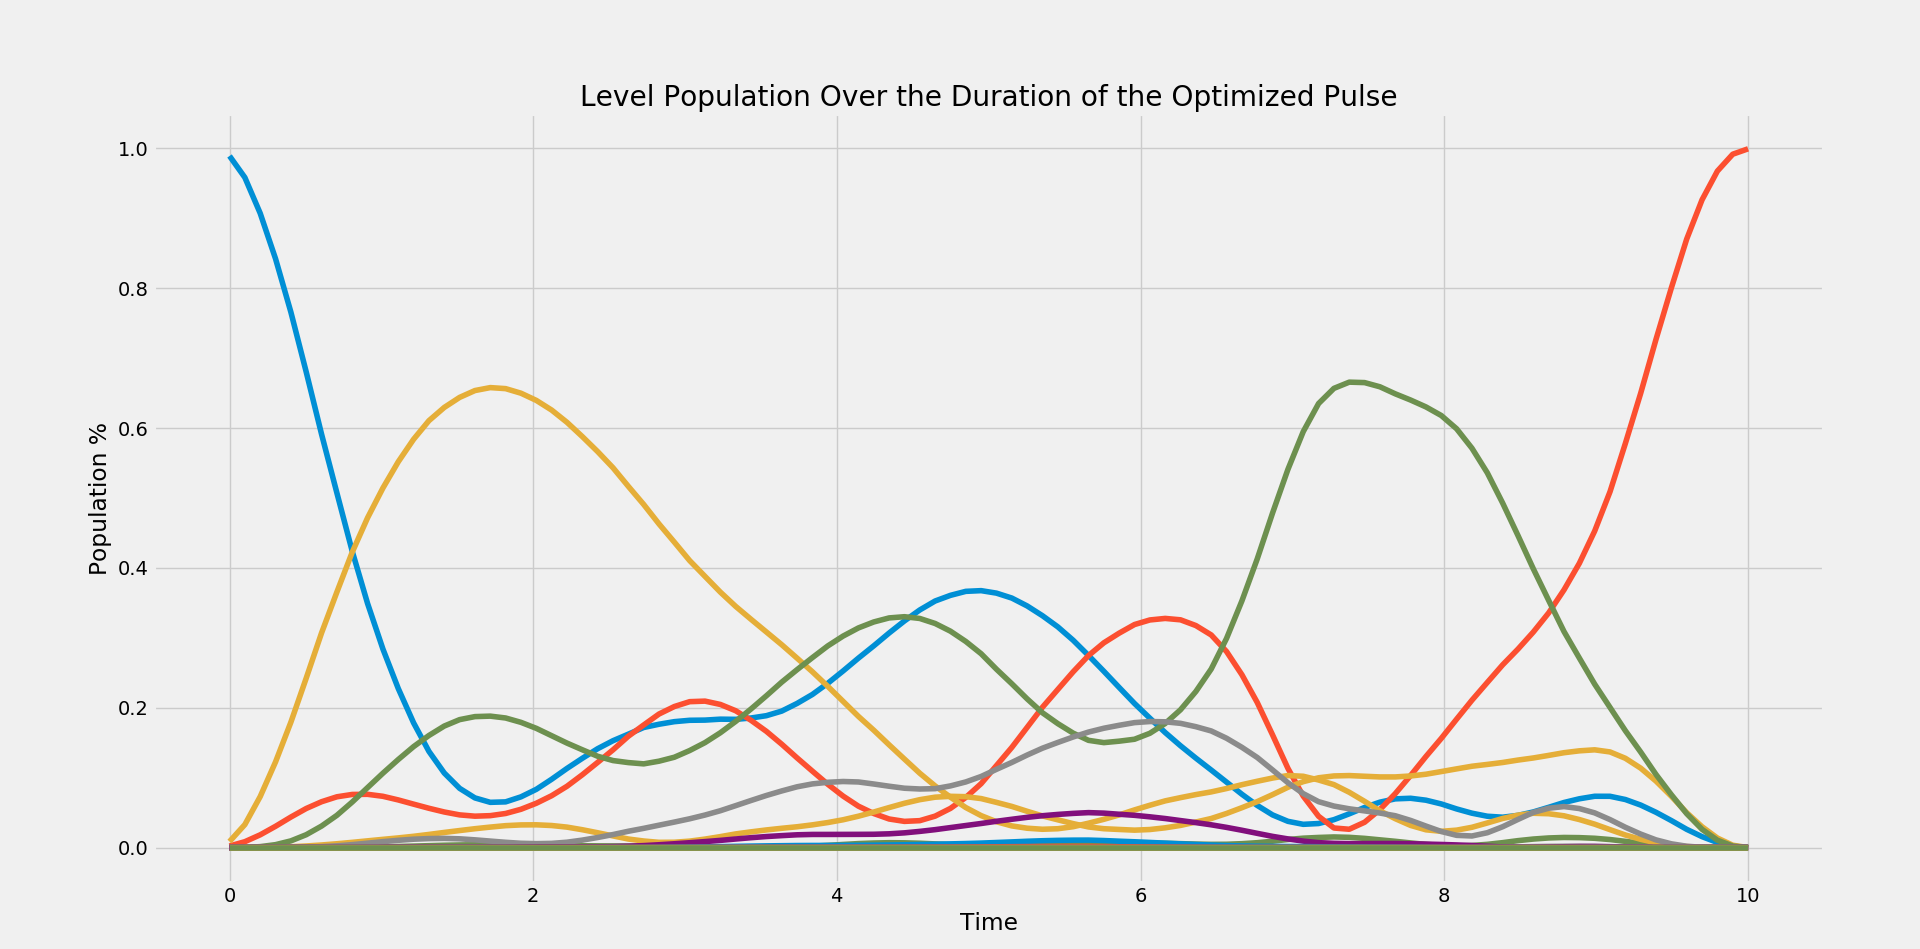
\includegraphics[width=1\columnwidth]{Results/transmon-cavity/g0-g1-level-population.png}
    \caption{Transmon-cavity state population over the duration of the pulse that does the transformation $\ket{g} \otimes \ket{0}\ \text{ (Blue)} \longrightarrow \ket{g} \otimes \ket{1}\ \text{ (Red)}$.}
    \label{fig:transmon-cavity-population}
\end{figure}
After you see this graph, you'd think that the constraint didn't work correctly. After all, the transformation is from level $\ket{0}$ to level $\ket{1}$, but there were many other levels that got occupied during the middle of the pulse. This is a valid guess, but there is an explanation why the higher level would get occupied. The reason is that you can't really create number states \textit{directly} in a cavity. You can only create coherent states \textit{directly}. To create  number state you need to make the coherent states interfere in a way that creates a number state.

So why then should this graph show it was successful then? Well, I ran the algorithm with 50 cavity levels (!), this means that there are actually 100 curves in that graph (50 of the cavity times 2 of the qubit). If you'd try to count the number of curves that you see you'll probably count 7-8 curves and not all of the 100, this is since most of the curves stay at zero population. This is exactly what we want, the higher levels don't affect the physics of the system, if we add more levels (like in the real world where there are infinite levels) the pulse would still give the same desired result.
% As you can see, although the final result is what we want it to be, along the way higher levels were created, even to last level of the cavity were excited. This is a problem since, as we said earlier, the cavity should have infinite levels and cutting it off after 7 levels in this case is just and approximation, the last levels should not be populated.

% We can now add the penalty and see that this problem is solved with it.

\subsection{Finding a Good Initial Guess}
Although the GRAPE algorithm is the one responsible to find to optimal control pulse, we still need to give it some initial guess and the algorithm does the rest. You might think that this isn't much of a problem since theoretically any initial guess should arrive at a desired result. The problem is that often the algorithm gets stuck and can't find a result. This could be caused by a number of reasons, the main two are when the constraints are too strong and when the initial guess is not good enough.

When the constraints are too strong, the algorithm might prefer optimizing them instead of the fidelity and what we get is a pulse that achieves horrible fidelity but within the constraints. The solution is simply weakening the constraints (choosing a smaller $\lambda$ for the constraint).

The other, harder to solve problem is when the initial guess of the pulse is problematic. For example, if you choose the initial guess to be the most obvious initial guess you can make, constant 0, the algorithm will probably stop after one iteration changing nothing. This is because the gradient of a constant 0 pulse is actually zero, so the optimization algorithm thinks it's in an optimized minimum when in fact, it couldn't be more wrong.

The other simple initial guess you might think of using is a random pulse. After all, we don't know what is the desired pulse so picking a random pulse is as good as any other. The problem with a random pulse is that it is not a smooth function, so the algorithm might find it difficult to get a smooth solution.

There are two approaches we can take to get a good initial pulse. The first approach assumes nothing about the system, it's good since it's really general and can be used in any case, but might be not ideal in some cases. The second approach is when we know roughly how the solution should look like, we can use some pulse that is similar to what we expect and GRAPE will get the actual pulse from that.

In the first approach, we want GRAPE to do most of the work, but not get stuck by some weird problem of the initial pulse. We want a guess that is close to 0, pretty random, but not so much that it would be hard to smoothen. We can get such a pulse by doing a convolution between a random pulse and a Gaussian window 
% TODO: Continue to expalian why these convolutions work and give and equation

Unlike the first approach, the second approach could look really different for different examples but I'll give some general guidelines you can use the get a good initial pulse. Let's say, for example, you have a 3-level system where the third level isn't wanted (such as in the DRAG example). If you give an initial guess like the one in the first approach, the third level will still be excited by that pulse, and it might be hard for the algorithm to fix this. What you might do in this scenario, is to start with an initial guess that you know excites only the first and second levels of the system but not the third. This is easy since you  know the transition frequencies of the atom, from that you know the frequency that excites each level. What you can do is some random pulse that has frequency around the first-second levels frequency difference. So if you look in the frequency space, what you see is some Gaussian distribution around the first levels frequency with some random noise on it.

\begin{figure}[H]
    \centering
    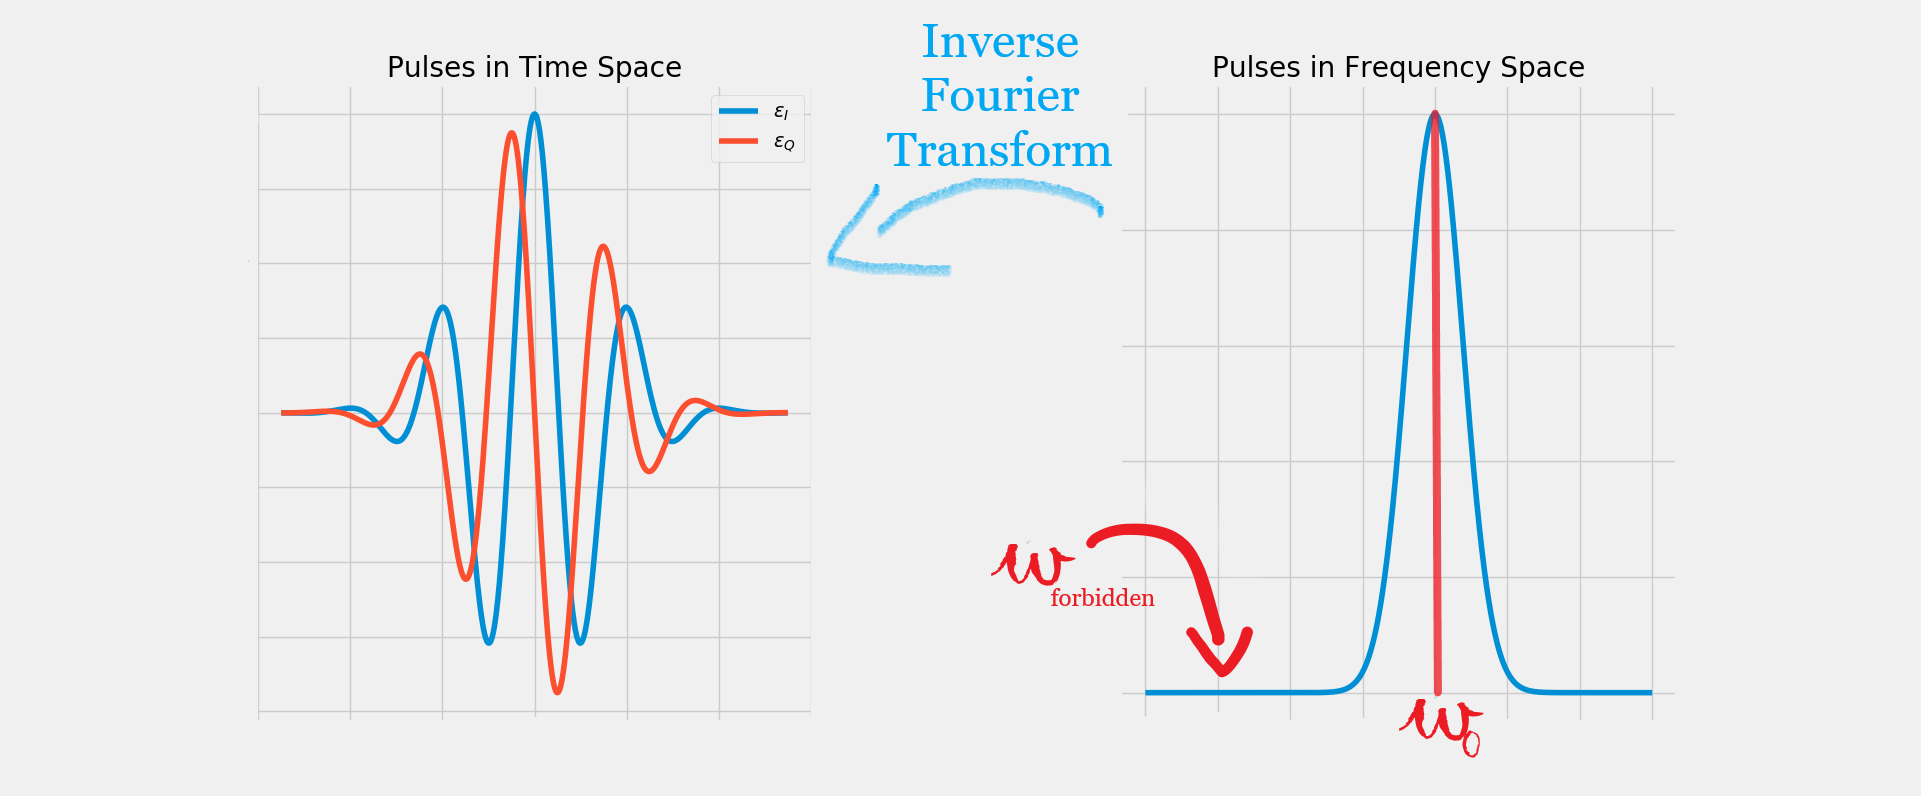
\includegraphics[width=1\columnwidth]{exaple-of-engineered-guess-edited.png}
    \caption{Example of how you might engineer an initial pulse for a system with known characteristics. Normally you would also add some random noise on top of the pulse}
    \label{fig:example-engineered-initial-guess}
\end{figure}
\subsection{From States to Gates}\label{sec:gate-GRAPE}
Until now we've discussed how to find pulses that take our system from one state to another. This is useful for initializing the quantum system in a desired state. However, the operation is not well defined if we start in a state other than the one the pulse was designed for. In contrast, a  numerically optimized quantum gate must perform a well defined unitary transformation on arbitrary states.

Here's the thing, turns out, you can change the algorithm just a little bit and get a GRAPE algorithm that gives you back the optimal pulses that realizes a desired \textit{quantum gate}, instead of just taking you from one state to another. 

To make such gate GRAPE, instead of optimizing for one state transformation, you optimize for  initial states that constitute a basis for the entire state space. This way, since quantum operations are linear, a unique transformation on the basis of the state space is a unique transformation on the entire system. The implementation of gate GRAPE is outside the scope of this project.

\subsection{References and Further Readings}
The best reference I've found on this subject is by far the 2019 dissertation of Philip Reinhold from Yale, "\textbf{Controlling Error-Correctable Bosonic Qubits}", especially the forth chapter. Another great resource is the documentation of the python library "\textbf{QuTiP}", which was used to create some of the graphs here, but it's documentation has some really nice explanations.
